% Лекц 8. Тасралтгүй чанар, Уламжлал
% Эх: latex/lectures/lec08-continuity-derivative.tex (scripts/latex_to_beamer.py-ээр хөрвүүлсэн)
% Frame бүр слайдад нэг (эсвэл allowframebreaks-аар хэд хэдэн) хуудас болно;
% хэвлэх хувилбарт frame-ийн хил харагдахгүй, текст үргэлжилсэн байна.

\MathLecture{8}{Тасралтгүй чанар, Уламжлал}

\section{Тасралтгүй функц}
\begin{frame}[allowframebreaks]{Тасралтгүй функц}
\begin{definition}[Цэг дээр тасралтгүй чанар]
$y=f(x)$ функцын хувьд  
$$\displaystyle \lim_{x\to a} f(x)=f(a)$$ бол $y=f(x)$ функцыг $x=a$ цэгт тасралтгүй гэнэ.
\end{definition}
\end{frame}

\begin{frame}[allowframebreaks]{Тасралтгүй функц}
\begin{definition}[Тасралтгүй функц]
$y=f(x)$ функц тодорхойлогдох мужийнхаа бүх цэг дээр тасралтгүй бол тасралтгүй функц гэнэ. Хэрэв $(a,b)$ завсрын бүх цэг дээр тасралтгүй бол $(a,b)$ дээр тасралтгүй гэнэ.
\end{definition}
\end{frame}

\begin{frame}[allowframebreaks]{Тасралтгүй функц}
\begin{definition}[Цэг дээрх тасралт] $y=f(x)$ функцын хувьд $x=a$ цэгт тасралтгүй чанар биелэхгүй бол ( өөрөөр хэлбэл 
$\displaystyle \lim_{x\to a} f(x)\neq f(a)$ ) $x=a$ цэгт тасралттай гэнэ.
\end{definition}
\end{frame}

\begin{frame}[allowframebreaks]{Тасралтгүй функц}
\begin{note}
$f$ функц $x=a$ цэгт тасралтгүй байх 3 нөхцөл:
\begin{enumerate}[label=\arabic*)]
\item $f(a)$ оршин (төгсгөлөг) байх.
\item $\displaystyle \lim_{x\to a} f(x)$ оршин (төгсгөлөг) байх.
\item $\displaystyle \lim_{x\to a} f(x)=f(a)$ байх.
\end{enumerate}
\end{note}
\end{frame}

\begin{frame}[allowframebreaks]{Тасралтгүй функц}
\begin{example}
$y=f(x)=x+1$ функц $x=1$ цэг дээр тасралтгүй, учир нь
\[
\lim_{x\to 1} f(x)=\lim_{x\to 1} (x+1)=2 \quad \text{ба} \quad f(1)=2.
\]
Иймээс $\displaystyle \lim_{x\to 1} f(x)=f(1)$ биелнэ.


Доорх зурагт $f(x)=x+1$ шулуун ба $x=1$ цэг дээрх $f(1)=2$ утгыг онцолж үзүүлэв.
\begin{center}
  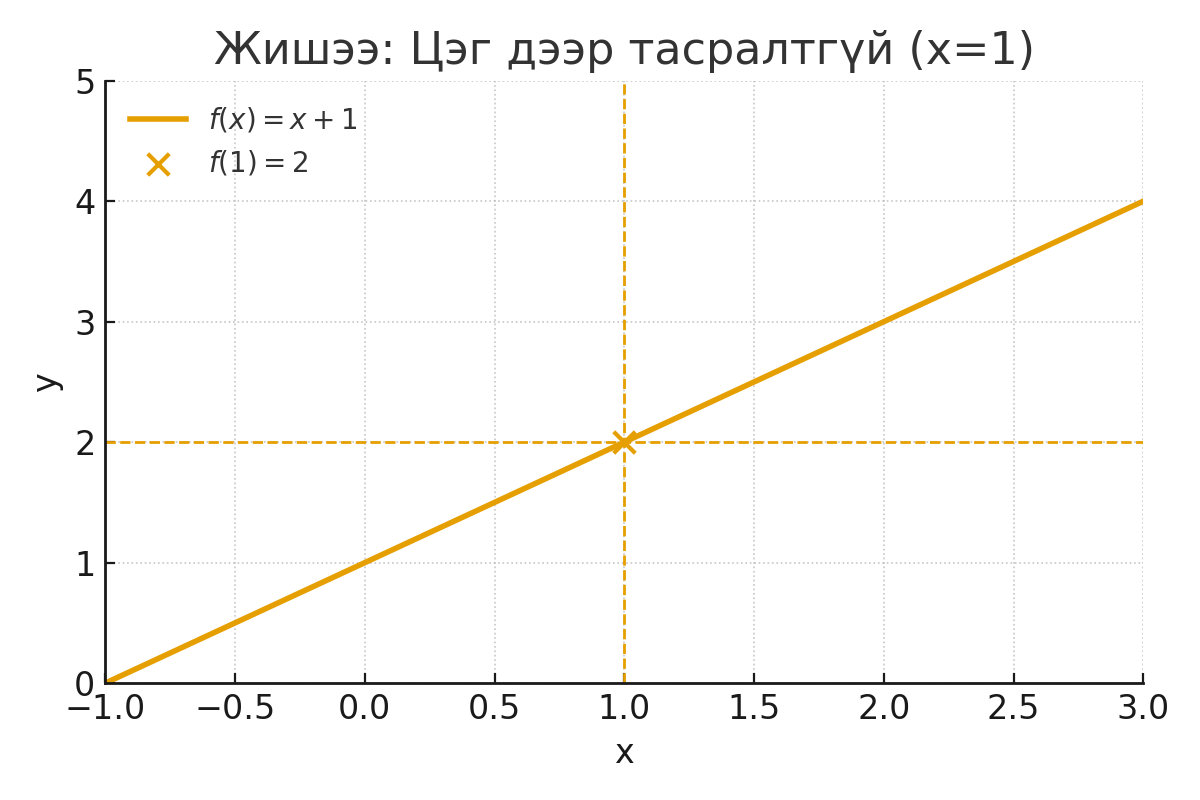
\includegraphics[width=.7\linewidth,max width=\linewidth,max height=.72\textheight]{continuous_at_point.png}
\end{center}
\end{example}
\end{frame}

\begin{frame}[allowframebreaks]{Тасралтгүй функц}
\begin{example}
\begin{remark}
Хэрэв 
$\displaystyle g(x)=\begin{cases}
\dfrac{x^2-1}{x-1}, & x\ne 1,\\
2, & x=1
\end{cases}$
тодорхойлбол $g(x)$ нь мөн $x=1$ дээр тасралтгүй болно, учир нь $g(x)=x+1$ байна.
\end{remark}
\end{example}
\end{frame}

\begin{frame}[allowframebreaks]{Тасралтгүй функц}
\begin{example}[Тасралтын жишээ]
\begin{enumerate}[label=\arabic*)]
\item $f(x)=\dfrac{1}{x^2}$ нь $(1,5)$ дээр тасралтгүй, харин $(-1,1)$ дээр $x=0$-д тодорхойлогдоогүй тул тасралттай.
\item $\displaystyle f(x)=\begin{cases}
\dfrac{x^2-3-\sqrt{x-1}}{x-2}, & x\ne 2,\\
3, & x=2
\end{cases}$ — $x=2$-д:
\begin{enumerate}[label=\alph*)]
\item $f(2)=3$.
\item $\displaystyle \lim_{x\to 2}\frac{x^2-3-\sqrt{x-1}}{x-2}
=\lim_{t\to 1}\frac{(t^2+1)^2-3-t}{t^2+1-2} = 3.5$ (орлуулалт $t=\sqrt{x-1}$).
\item $f(2)\ne \lim\limits_{x\to 2} f(x)$ тул тасралттай. (Хэрэв $f(2)=3.5$ бол тасралтгүй байна.)
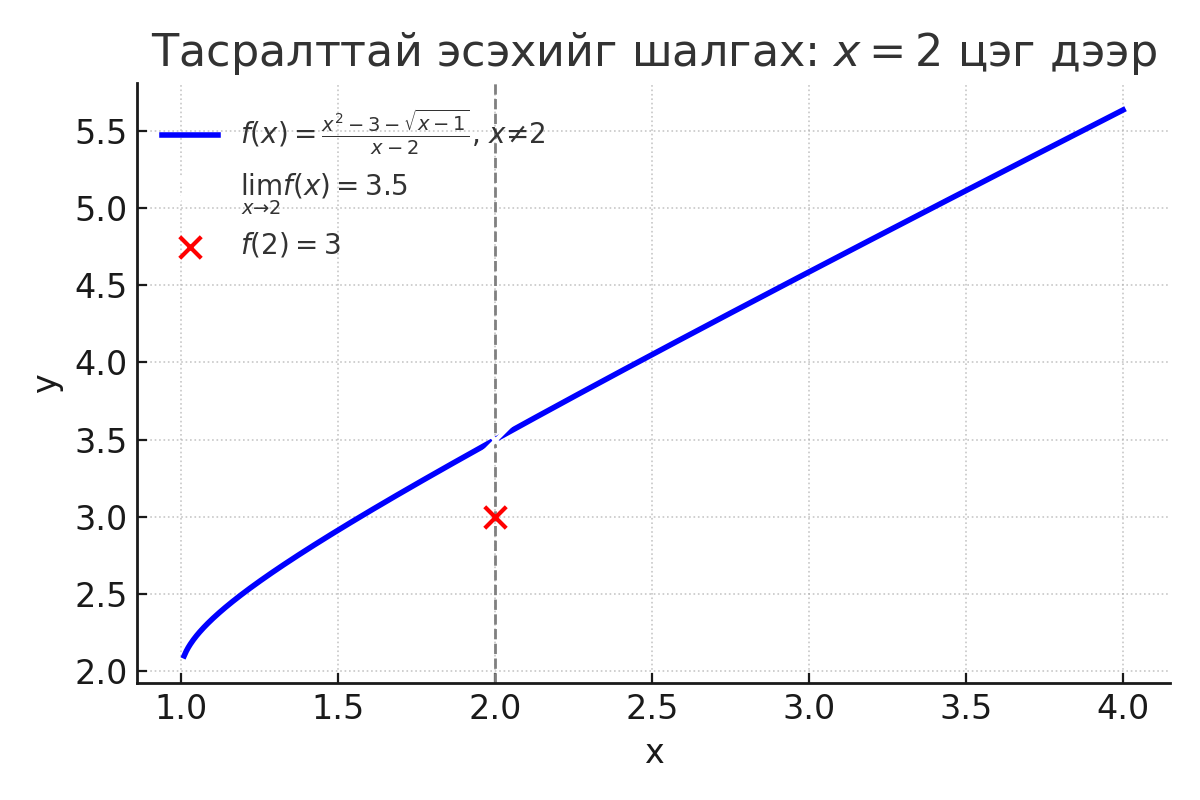
\includegraphics[scale=0.7,max width=\linewidth,max height=.72\textheight]{continuity_x2_case_white_dot.png}
\end{enumerate}
\end{enumerate}
\end{example}
\end{frame}

\begin{frame}[allowframebreaks]{Тасралтгүй функц}
\begin{theorem}[Арифметик үйлдлүүд] Хэрэв $f, g$ нь $x=a$-д тасралтгүй бол $f\pm g$, $f\cdot g$, мөн $g(a)\ne 0$ үед $\dfrac{f}{g}$ нь $x=a$-д тасралтгүй.
\end{theorem}
\end{frame}

\begin{frame}[allowframebreaks]{Тасралтгүй функц}
\begin{theorem}[Композици] Хэрэв $g$ нь $x=a$-д, $f$ нь $x=g(a)$-д тасралтгүй бол $f\circ g$ нь $x=a$-д тасралтгүй.
\end{theorem}
\end{frame}

\begin{frame}[allowframebreaks]{Тасралтгүй функц}
\begin{theorem}[Урвуу функц] Хэрэв $f$ урвуутай бөгөөд $x=a$-д тасралтгүй бол $f^{-1}$ нь $x=f(a)$-д тасралтгүй.
\end{theorem}
\end{frame}

\section{Өөрчлөлтийн харьцаа ба шүргэгч шулуун}
\begin{frame}[allowframebreaks]{Өөрчлөлтийн харьцаа ба шүргэгч шулуун}
\begin{definition}[Өөрчлөлтийн харьцаа]
$a,b$ нь $a\ne b$ тогтмол тоонууд байг. $y=f(x)$ функцийг $x=a$-аас $x=b$ хүртэл өөрчлөхөд
\[
\Delta x=b-a,\qquad \Delta y=f(b)-f(a),
\]
\[
\frac{\Delta y}{\Delta x}=\frac{f(b)-f(a)}{b-a}
\]
-ийг $f(x)$ функцийн $[a,b]$ дээрх өөрчлөлтийн харьцаа гэнэ. Энэ нь $A(a,f(a))$ ба $B(b,f(b))$ цэгүүдийг дайрсан \emph{хөвч} шулууны налалт юм.
\end{definition}
\end{frame}

\begin{frame}[allowframebreaks]{Өөрчлөлтийн харьцаа ба шүргэгч шулуун}
\begin{example}
$f(x)=x^2$ функцийн хувьд
\begin{enumerate}
  \item $x=-1$-ээс $x=2$ хүртэл: $\dfrac{\Delta y}{\Delta x}=\dfrac{2^2-(-1)^2}{2-(-1)}=\dfrac{3}{3}=1$.
  \item $x=a$-аас $x=a+h$ хүртэл: $\dfrac{(a+h)^2-a^2}{h}=2a+h$.
\end{enumerate}
\end{example}
\end{frame}

\section{Уламжлалын тодорхойлолт ба тэмдэглэгээ}
\begin{frame}[allowframebreaks]{Уламжлалын тодорхойлолт ба тэмдэглэгээ}
\begin{definition}[Цэг дээрх уламжлал]
$f$ функц $x=a$ цэгийн орчимд тодорхойлогдсон байг. Хэрэв
\[
\lim_{h\to 0}\frac{f(a+h)-f(a)}{h}
\]
хязгаар оршин байвал $f$ нь $x=a$ \textbf{цэг дээр дифференциалчлагдана} гэнэ; уг хязгаарыг $f'(a)$ буюу цэг дээрх уламжлал гэнэ.
\end{definition}
\end{frame}

\begin{frame}[allowframebreaks]{Уламжлалын тодорхойлолт ба тэмдэглэгээ}
\begin{note}
Цэг дээрх уламжлал $f'(a)$ нь $A(a,f(a))$ цэг дээр татсан шүргэгч шулууны налалт бөгөөд шүргэгчийн тэгшитгэл:
\[
y - f(a) = f'(a)\,(x-a).
\]
\end{note}
\end{frame}

\begin{frame}[allowframebreaks]{Уламжлалын тодорхойлолт ба тэмдэглэгээ}
\begin{example}
$f(x)=x^2-2x-1$ үед
\[
f'(3)=\lim_{h\to 0}\frac{f(3+h)-f(3)}{h}
=\lim_{h\to 0}\frac{(3+h)^2-2(3+h)-1 - (9-6-1)}{h}=4.
\]
\end{example}

\begin{center}
\begin{fitbox}\begin{tikzpicture}[scale=1]
  % Axes
  \draw[->] (-1,0) -- (5,0) node[right] {$x$};
  \draw[->] (0,-4) -- (0,6) node[above] {$y$};

  % f(x)=x^2-2x-1
  \draw[thick] plot[samples=200,domain=-0.2:4.5] (\x,{(\x*\x - 2*\x - 1)}) node[right] {$y=f(x)=x^2-2x-1$};

  % a=3 point
  \coordinate (P) at (3,{(3*3 - 2*3 - 1)});
  \fill (P) circle (2pt) node[above right] {$A(3,f(3))$};

  % tangent at x=3: f'(x)=2x-2 => f'(3)=4 ; y - f(3)=4(x-3)
  \draw[very thick,red] (1,{2+4*(1-3)}) -- (4.5,{2+4*(4.5-3)}) node[above right] {шүргэгч};

  % A few secants approaching tangent: pick b=3+h
  \foreach \h/\col in {1/blue,0.5/blue,0.25/blue}{
    \coordinate (B) at ({3+\h},{(3+\h)*(3+\h)-2*(3+\h)-1});
    \draw[\col] (P) -- (B);
    \fill (B) circle (1.5pt);
  }
\end{tikzpicture}\end{fitbox}
\end{center}
\end{frame}

\subsection*{Тэмдэглэгээ}
\begin{frame}[allowframebreaks]{Тэмдэглэгээ}
$y=f(x)$ бол $f'(x)$, $\dfrac{dy}{dx}$, $Df(x)$, $y'$ зэрэг тэмдэглэгээг хэрэглэнэ.
\end{frame}

% Семинар ба гэрийн даалгавар (Берманы бодлогын хураамжаас)
% Лекц 8: семинар ба гэрийн даалгавар. Бодлогууд: Г.Н. Берман, "Сборник задач по курсу
% математического анализа" (22-р хэвлэл). [Б.N] нь номын бодлогын дугаар.

\ProblemSet{Семинар 8}
\begin{frame}[allowframebreaks]{Семинар 8}
\pgroup{Тасралтгүй чанар ба тасралтын цэг.}
\begin{plist}
\prob{221}{$y=0$ \ ($x<0$), \ $y=x$ \ ($0\le x<1$), \ $y=-x^2+4x-2$ \ ($1\le x<3$), \ $y=4-x$ \ ($x\ge3$) функц тасралтгүй юу?}
\prob{223}{$f(x)=x+1$ \ ($x\le1$), \ $f(x)=3-ax^2$ \ ($x>1$). $a$-г ямар байхад $f$ тасралтгүй болох вэ? Графикийг байгуул.}
\prob{224}{$f(x)=-2\sin x$ \ ($x\le-\frac{\pi}{2}$), \ $A\sin x+B$ \ ($-\frac{\pi}{2}<x<\frac{\pi}{2}$), \ $\cos x$ \ ($x\ge\frac{\pi}{2}$). $f$ тасралтгүй байхаар $A,B$-г сонго.}
\prob{225}{$y=\frac{1}{x-2}$ ба $y=\frac{1}{(x+2)^2}$ функцүүд ямар цэгүүдэд тасрах вэ? Тасралтын цэгийн орчим дахь төлөвийн ялгааг тайлбарла.}
\prob{226}{$f(x)=\frac{x^2-1}{x^3-1}$ функц $x=1$ дээр тодорхойлогдоогүй. $x=1$ дээр тасралтгүй болгохын тулд $f(1)$ ямар байх ёстой вэ?}
\prob{227}{$y=\frac{\sin x}{x}$ ба $y=\frac{\cos x}{x}$ функцүүд $x=0$ дээр ямар төрлийн тасралттай вэ?}
\prob{228}{$y=\frac{|x|}{x}$ \ ($x\ne0$), \ $y=0$ \ ($x=0$) функцийн тасралтгүй чанарыг шинжилж, графикийг байгуул.}
\prob{230}{$y=\arctg\frac1x$ функцийг $x=0$ дээр тасралтгүй болгож дутуу тодорхойлж болох уу?}
\prob{232}{$f(x)=x\sin\frac{\pi}{x}$. Хаа сайгүй тасралтгүй байхын тулд $f(0)$ ямар байх ёстой вэ?}
\end{plist}
\pgroup{Уламжлалын тодорхойлолт.}
\begin{plist}
\prob{440}{$y=x^3$ функцийн $x_1=2$ цэг дээрх өөрчлөлтийг $\Delta x=2;\ 1;\ 0{,}5;\ 0{,}1$ үед ол.}
\prob{441.1}{$y=2x^3-x^2+1$, \ $x=1$, \ $\Delta x=0{,}1$ үед $\frac{\Delta y}{\Delta x}$-г олж, $\Delta x\to0$ үед хязгаар нь 4 болохыг харуул.}
\prob{443}{$f(x)=x^2$; \ $f'(5),\ f'(-2),\ f'\bigl(-\frac32\bigr)$-г тодорхойлолтоор ол.}
\prob{447}{$y=\sin x$ функцийн $x=0$ дээрх уламжлалыг тодорхойлолтоор ол.}
\prob{453}{Тэгш функцийн уламжлал сондгой, сондгой функцийн уламжлал тэгш функц болохыг батал.}
\prob{907}{$y=|x|$ функц $x=0$ дээр тасралтгүй боловч дифференциалчлагдахгүйг харуул.}
\end{plist}
\pgroup{Уламжлалын геометр утга.}
\begin{plist}
\prob{454}{$y=x^2$ параболын 1) координатын эх, 2) $(3;9)$, 3) $(-2;4)$ цэгүүд, 4) $y=3x-2$ шулуунтай огтлолцох цэгүүд дээрх шүргэгчийн өнцгийн коэффициентийг ол.}
\prob{456}{$y=x^2$ параболын ямар цэг дээрх шүргэгч 1) $Ox$ тэнхлэгтэй параллель, 2) $Ox$ тэнхлэгтэй $45^\circ$ өнцөг үүсгэх вэ?}
\prob{459}{$y=x^2$ ба $y^2=x$ параболууд ямар өнцгөөр огтлолцох вэ?}
\prob{461}{$y=x^3$ муруйн абсцисс нь 2 байх цэг дээрх шүргэгч ба нормалийн тэгшитгэлийг бич.}
\prob{463}{$y=x^2$ параболын ямар цэг дээрх шүргэгч 1) $y=4x-5$ шулуунтай параллель, 2) $2x-6y+5=0$ шулуунтай перпендикуляр, 3) $3x-y+1=0$ шулуунтай $45^\circ$ өнцөг үүсгэх вэ?}
\end{plist}
\end{frame}

\ProblemSet{Гэрийн даалгавар 8}
\begin{frame}[allowframebreaks]{Гэрийн даалгавар 8}
\pgroup{Тасралтгүй чанар ба тасралтын цэг.}
\begin{plist}
\prob{222}{Суурийн радиус нь 3, 2, 1 м, өндөр нь бүгд 5 м байх гурван цилиндрийг бие биен дээр нь тавив. Үүссэн биетийн хөндлөн огтлолын талбайг доод цилиндрийн доод суурь хүртэлх зайн функцээр илэрхийл. Энэ функц тасралтгүй юу? Графикийг байгуул.}
\prob{229}{$y=\frac{1}{\lg|x|}$ функц хэдэн тасралтын цэгтэй, ямар төрлийнх вэ? Графикийг байгуул.}
\prob{231}{$f(x)=\sin\frac{\pi}{2x}$ \ ($x\ne0$), \ $f(0)=1$ функцийн тасралтгүй чанарыг шинжил.}
\prob{233}{$y=\frac{1}{1+2^{1/x}}$ функц $x=0$ дээр I төрлийн тасралттайг батал.}
\prob{234}{$y=2^{-2^{1/(1-x)}}$ функцийн $x=1$ дээрх тасралтын төрлийг тогтоо. $x=1$ дээр тасралтгүй болгож тодорхойлж болох уу?}
\prob{235}{$y=\frac{2^{1/x}-1}{2^{1/x}+1}$ функцийн $x=0$ дээрх тасралтын төрлийг тогтоо.}
\prob{236}{$f(x)=(x+1)\,2^{-\left(\frac{1}{|x|}+\frac1x\right)}$ \ ($x\ne0$), \ $f(0)=0$. $[-2,2]$ дээр $f$ нь $f(-2)$ ба $f(2)$-ын хоорондох бүх утгыг авдаг боловч тасралттайг харуул (аль цэгт?).}
\prob{237}{$y=\frac{1}{1+2^{\tg x}}$ функцийн тасралтгүй чанарыг шинжил.}
\prob{238}{$x$ рационал бол $f(x)=0$, иррационал бол $f(x)=x$. $f$ ямар цэгт тасралтгүй вэ?}
\end{plist}
\pgroup{Уламжлалын тодорхойлолт.}
\begin{plist}
\prob{441.2}{$y=\frac1x$, \ $x=2$, \ $\Delta x=0{,}01$ үед $\frac{\Delta y}{\Delta x}$-г олж, $\Delta x\to0$ үед хязгаар нь $-\frac14$ болохыг харуул.}
\prob{442}{$y=x^2$ функцийн $x=3$ дээрх уламжлалын ойролцоо утгыг $\Delta x=0{,}5;\ 0{,}1;\ 0{,}01;\ 0{,}001$ үед ол.}
\prob{444}{$f(x)=x^3$; \ $f'(1),\ f'(0),\ f'(-\sqrt2),\ f'\bigl(\frac13\bigr)$-г ол.}
\prob{445}{$f(x)=x^2$. Ямар цэгт $f(x)=f'(x)$ байх вэ?}
\prob{446}{$f(x)=x^2$ функцийн хувьд $f'(a+b)=f'(a)+f'(b)$ биелэхийг шалга. $f(x)=x^3$-ийн хувьд биелэх үү?}
\prob{448}{$y=\lg x$ функцийн $x=1$ дээрх уламжлалыг ол.}
\prob{449}{$y=10^x$ функцийн $x=0$ дээрх уламжлалыг ол.}
\prob{450}{$f(0)=0$ ба $x\to0$ үед $\frac{f(x)}{x}$-ийн хязгаар оршин байдаг. Энэ хязгаар $f'(0)$-тэй тэнцүүг батал.}
\prob{451}{$f(0)=\varphi(0)=0$, $x=0$ дээр уламжлалтай, $\varphi'(0)\ne0$ бол $\displaystyle\lim_{x\to0}\frac{f(x)}{\varphi(x)}=\frac{f'(0)}{\varphi'(0)}$ болохыг батал.}
\prob{452}{$f(x)$ нь $x=a$ дээр уламжлалтай бол $\displaystyle\lim_{x\to a}\frac{xf(a)-af(x)}{x-a}=f(a)-af'(a)$ болохыг батал.}
\prob{908}{$y=|x^3|$ функцийн $x=0$ дээрх тасралтгүй ба дифференциалчлагдах чанарыг шинжил.}
\prob{909}{$f(x)=1+x$ \ ($x\le0$), \ $x$ \ ($0<x<1$), \ $2-x$ \ ($1\le x\le2$), \ $3x-x^2$ \ ($x>2$). $f$-ийн тасралтгүй чанарыг шинжилж, $f'(x)$ оршин байх ба тасралтгүй эсэхийг тогтоо.}
\end{plist}
\pgroup{Уламжлалын геометр ба физик утга.}
\begin{plist}
\prob{455}{$y=x^3$ кубын параболын ямар цэгүүдэд шүргэгчийн өнцгийн коэффициент 3-тай тэнцүү вэ?}
\prob{457}{$y=x^3$ кубын параболын шүргэгч $Ox$ тэнхлэгтэй мохоо өнцөг үүсгэж болох уу?}
\prob{458}{$y=x^2$ парабол ба $3x-y-2=0$ шулуун ямар өнцгөөр огтлолцох вэ?}
\prob{460}{$y=\frac1x$ гипербол ба $y=\sqrt x$ парабол ямар өнцгөөр огтлолцох вэ?}
\prob{462}{Аргументын ямар утгад $y=x^2$ ба $y=x^3$ муруйнуудын шүргэгчүүд параллель байх вэ?}
\prob{464}{$y=ax^2$ параболын дурын цэг дээрх дэд шүргэгч нь шүргэлтийн цэгийн абсциссын хагастай тэнцүүг батал. Үүнийг ашиглан шүргэгч байгуулах аргыг заа.}
\prob{432}{$AB$ нимгэн жигд бус саваа $L=20$ см урттай. $AM$ хэсгийн масс $M$ цэгээс $A$ хүртэлх зайн квадраттай пропорционал, $AM=2$ см хэсгийн масс 8 г. 1) $AM=2$ см хэсгийн дундаж нягт, 2) бүх савааны дундаж нягт, 3) $M$ цэг дэх нягтыг ол.}
\prob{433}{30 см урт $AB$ саваанд масс (граммаар) $m=3l^2+5l$ хуулиар тархсан ($l$ нь $A$-аас тоолсон урт). 1) Савааны дундаж шугаман нягт, 2) $l=5$ см цэг, $A$ цэг, савааны төгсгөл дэх нягтыг ол.}
\prob{434}{1 кг усыг $0$-ээс $t^\circ$C хүртэл халаах дулааны хэмжээ $Q=4186{,}8(t+0{,}00002t^2+0{,}0000003t^3)$ Ж. $t=30^\circ$ ба $t=100^\circ$ үеийн усны дулаан багтаамжийг ($Q'(t)$) ол.}
\end{plist}
\end{frame}

